\chapter{Setup and Samples}
In this Chapter I will introduce the design and preparation of my samples. Then I will introduce the cryostats and magnets, the vector network analyzer including signal pre-amplifier, and finally discuss the sample holder and cabling used in my experiments.

%%%%%%%%%%%%%%%%%%%%%%%%%%%%%%%%%%%%%%%%%%%%%%%%%%%%%%%%%%%%%%%%%%%%%%%%%%%%%%%%%%%%%%%%%%%%%%%
\section{Sample Design and Preparation} \label{sec:sample_design} 
First, as already shown in Chapter \ref{sec:coherence_length}, the thickness of the Co should be somewhere between $3.7$ to $52\,$nm to be able to measure a significant difference in electronic transport between singlet and triplet superconductivity. At the same time I prefer a sample volume as large as possible, since a large volume also means a considerable absorption and thus a ferromagnetic resonance (FMR) signal. Therefore, it seemed advisable to start with a Co layer of $30\,$nm.

To complete the superconductor/ferromagnet/superconductor (S/F/S) contact, I use $100\,$nm Al each to sandwich the Co. Here I study the thicknesses already used by Andreas Bloch for the electronic transport measurement optimized samples.

Since we are also interested in transport measurements through the S/F/S contact, we had to prevent it from being short-circuited. Therefore, the S/F/S contact must be electrically isolated from the co-planar wave guide (CPW) on top. This was achieved by an intermediate polyimide (PI) layer.

The CPW on the top of the samples consists of an inner conductor and ground pads. It is composed of a thin layer of Ti for good adhesion with a thick layer of Au for high conductivity on top. Figure \ref{fig:sample_wg} shows a schematic diagram of the top view and the dimensions used.
\begin{figure}
     \centering
     \begin{subfigure}[b]{.45\textwidth}
         \centering
         \import{setup/sample}{cobulk30nm.pdf_tex}
         %Au $50\,$nm\\Ti $3\,$nm\\PI $1\,$\textmu m\\Al $100\,$nm\\Co $30\,$nm\\Al $100\,$nm\\Si wafer
         \caption{Sample schematic CPW1}
         \label{fig:sample_cobulk30nm}
     \end{subfigure}
     \begin{subfigure}[b]{.45\textwidth}
         \centering
         \import{setup/sample}{CoBulky32nm.pdf_tex}
         \caption{Sample schematic CPW2}
         \label{fig:sample_cobulky32nm}
     \end{subfigure}
     \begin{subfigure}[b]{.45\textwidth}
         \centering
         \import{setup/sample}{cpw8.pdf_tex}
         %Au $50\,$nm\\Ti $5\,$nm\\$\downarrow$ Al$_2$O$_3$\\Al $120\,$nm\\Co $3\,$nm\\Si wafer
         \caption{Sample schematic CPW3}
         \label{fig:sample_cpw456}
     \end{subfigure}
     \begin{subfigure}[b]{.45\textwidth}
         \centering
         \import{setup/sample}{wave-guide.pdf_tex}
         \caption{Sample schematic top-view}
         \label{fig:sample_wg}
     \end{subfigure}
        \caption[Schematics of the sample designs]{Schematics of the different sample designs. \textbf{(a)}, \textbf{(b)} \& \textbf{(c)} are showing the cross-sections of the samples CPW1, CPW2 \& CPW3. On each right side, the different materials and thicknesses are written. In \textbf{(d)} you can see a top-view of the used wave guide mask and its dimensions. These dimensions are used for all my samples.}
        \label{fig:sample}
\end{figure}

The samples CPW1 (Figure \ref{fig:sample_cobulk30nm}) and CPW2 (Figure \ref{fig:sample_cobulky32nm}) consist of a S/F/S sandwich structure of Al/Co/Al, a PI layer and a Ti/Au CPW on top. They differ slightly in the Co thickness and in the lateral extent of the Al/Co/Al sandwich. While the sandwich on the CPW1 sample is extended over the whole chip, the sandwich on the CPW2 sample is structured in the shape of the CPW.

It has turned out that smaller layers of Co, such as $3\,$nm, are also very interesting. Here singlet superconductivity can be studied easily, but also the effect of triplet superconductivity will be investigable. The sample CPW3 (Figure \ref{fig:sample_cpw456}) consists of a single sandwich in the shape of the CPW. At the very bottom is a 3nm Co layer directly on the wafer to get the Co layer as continuous as possible. On top of that is a Cu\footnote{Cu was used to rule out Zeeman splitting in aluminum, as a cause of parts of the signal. However, hypothesis of Zeeman splitting was proven to be wrong.} layer and a Ti/Au CPW.

Now I would like to go through the preparation steps using sample CPW2. Used parameters can be found in Table \ref{tab:setup_sampleprep}, in the Appendix. For photo-lithography a layer of photoresist is deposited on a Si wafer. The resist is exposed to UV light in the form of the CPW by the mask-less photo-lithography tool. The resist is then developed and the sample is covered with the Al/Co/Al sandwich either by thermal or electron-beam evaporation. During lift-off, the remaining resist layer with the Al/Co/Al sandwich on top comes off. Now an Al/Co/Al sandwich structure in the form of a CPW remains. After applying a PI layer, the lithography process just described is repeated for a Ti/Au layer instead of Al/Co/Al. 
%%%%%%%%%%%%%%%%%%%%%%%%%%%%%%%%%%%%%%%%%%%%%%%%%%%%%%%%%%%%%%%%%%%%%%%%%%%%%%%%%%%%%%%%%%%%%%%
\section{Setup} \label{sec:setup_setup}
In this Section I want to describe the two setups 'BlueFors' and 'HelioxVL', I used. A schematic for each setup can be found in Figure \ref{fig:setup_schematic}. A list of the used devices, can be found in Table \ref{tab:setup_setup}.
\begin{figure}
     \centering
     \begin{subfigure}[b]{.45\textwidth}
         \centering
    \import{setup/messschema}{messschema12.pdf_tex}
         \caption{BlueFors setup schematic}
         \label{fig:setup_schematic_bluefors}
     \end{subfigure}
     \begin{subfigure}[b]{.45\textwidth}
         \centering
    \import{setup/messschema}{messschema21.pdf_tex}
         \caption{HelioxVL setup schematic}
         \label{fig:setup_schematic_heliox}
     \end{subfigure}
        \caption[Schematics of the two setups]{Schematics of the two used setups. In the \textbf{\color{antiseeblau65}magenta} boxes the temperature can be set, to the indicated \textbf{\color{antiseeblau65}$\mathbf{4}\,$K} or \textbf{\color{antiseeblau65}$\boldsymbol{T}_\text{base}$}. The \textbf{\color[rgb]{0.49803922,0.49803922,0.49803922}grey} full circles are indicating the thermometers, which are measuring \textbf{\color[rgb]{0.49803922,0.49803922,0.49803922}$\boldsymbol{T}_\text{FMR}$}, \textbf{\color[rgb]{0.49803922,0.49803922,0.49803922}$\boldsymbol{T}_\text{M}$} \& \textbf{\color[rgb]{0.49803922,0.49803922,0.49803922}$\boldsymbol{T}_\text{RT}$}. The \textbf{\color{seeblau100}blue} color indicates the high-frequency part. It contains the device under testing (DUT), dampers, a pre-amplifier and the vector network analyzer (VNA). The \textbf{\color{seeblau65}light blue} color indicates the magnet coils and its controller. In addition the three programs {\color{seeblau100}'FMR control'}, {\color[rgb]{0.49803922,0.49803922,0.49803922}'LSCI 370'} and {\color{antiseeblau65}'Valve control'} are connected to the corresponding devices.}
        \label{fig:setup_schematic}
\end{figure}
\begin{table}
    \centering
    \caption{Devices used at BlueFors or HelioxVL setup}
    \vspace{4mm}
    \begin{tabular}{l|l}
     \hline BlueFors & 'BF-LD400' by 'BlueFors Oy' \cite{LD400manual}\\
         & stable temperature points: $4\,$K, $\approx 95\,$mK (specified: $8\,$mK)\\\hline
     magnet & 'AM430' by 'American Magnetics, Inc.' \cite{AM430manual}\\
     & $H_\text{max}=7\,$T, $\Delta H=0.5\,$mT\\\hline
     thermometer & 'LakeShore 370AC' by 'Lake Shore Cryotronics' \cite{LS370manual}\\
     & (incl. channel scanner 'LakeShore Model 3716')\\
     & $T_\text{FMR}$ range: $10\,$mK to $100\,$K ('RX-102B-CB') \cite{RX102bmanual}\\
     \vspace{5mm}& $T_\text{magnet}$ range: $4\,$K to RT (built-in)\\\hline
     
     HelioxVL & 'HelioxVL' by 'Oxford Instruments' \cite{HelioxVLmanual}\\
     & stable at: $4\,$K, $\approx 300\,$mK\\\hline
     magnet &  'IPS120-10' by 'Oxford Instruments' \cite{IPS12010manual}\\
     & $H_\text{max}=12\,$T, $\Delta H=1\,$mT\\\hline
     thermometer & 'LakeShore 370AC' by 'Lake Shore Cryotronics' \cite{LS370manual}\\
     \vspace{5mm}& $T_\text{FMR}$ range: $300\,$mK to RT ('CX-1010') \cite{CX1010manual}\\\hline
     
    VNA & 'R\&S$^\text{\textregistered}\,$ZNB40, variant 82'  by 'R\&S GmbH \& Co. KG' \cite{ZNB40manual, ZNB40spec, ZNB40brochure}\\
    & $f$ range: $100\,$kHz to $40\,$GHz\\
    & $P_\text{out}$ range: $-5$ to $-30\,$dB\\
    & $P_\text{in}$ range: $25$ to $-140\,$dB\\\hline
    pre-amplifier & 'U7227F/8C' by 'Keysight Technologies' \cite{U7227manual}\\
    & $P_\text{gain}=+17\,$dB\\\hline
    thermometer & 'GIR 2002' by 'Greisinger electronic GmbH' \cite{GIR2002manual, GMH3manual}\\
    & $T_\text{RT}$ range: $-200\,$C$^\circ$ to $1350\,$C$^\circ$ (thermocouple, type K)\\
    \end{tabular}
    \label{tab:setup_setup}
\end{table}

The BlueFors setup consists of a cryogen-free dilution refrigerator system with and a superconducting magnet. A large number of thermometers are also installed, although only two of them are used for measurements. One thermometer is installed in the magnet ($T_\text{magnet}$), the other one is mounted close to the sample holder ($T_\text{FMR}$), see Figure \ref{fig:setup_photo}a and has already been calibrated by Martin Prestel.

The cabling from the mixing chamber (MXC) to the sample holder was done previously by Sergej Andreev. At the $50\,$K stage, a damper for each measurement line with $-10\,$dB is mounted. Between the $4\,$K stage and the MXC, high-temperature superconducting cables are used. This choice ensures good electrical contact and reduces thermal contact between the stages. Additionally, connectors are screwed into each stage to ensure thermalization of the cables. Between mixing chamber and sample holder copper coaxial cables are used to ensure good thermal flow towards the sample. The sample holder is designed in such a way, that the inner conductor is simply pressed onto a PCB board. This procedure avoids ferromagnetic contamination by the typically used connectors. The PCB board clamps the sample down and connects the CPW to the high-frequency cables by CuBe alloy clamps. You can see a picture of the sample holder in Figure \ref{fig:setup_photo_bluefors}.
\begin{figure}
     \centering
     \begin{subfigure}[b]{.45\textwidth}
         \centering
         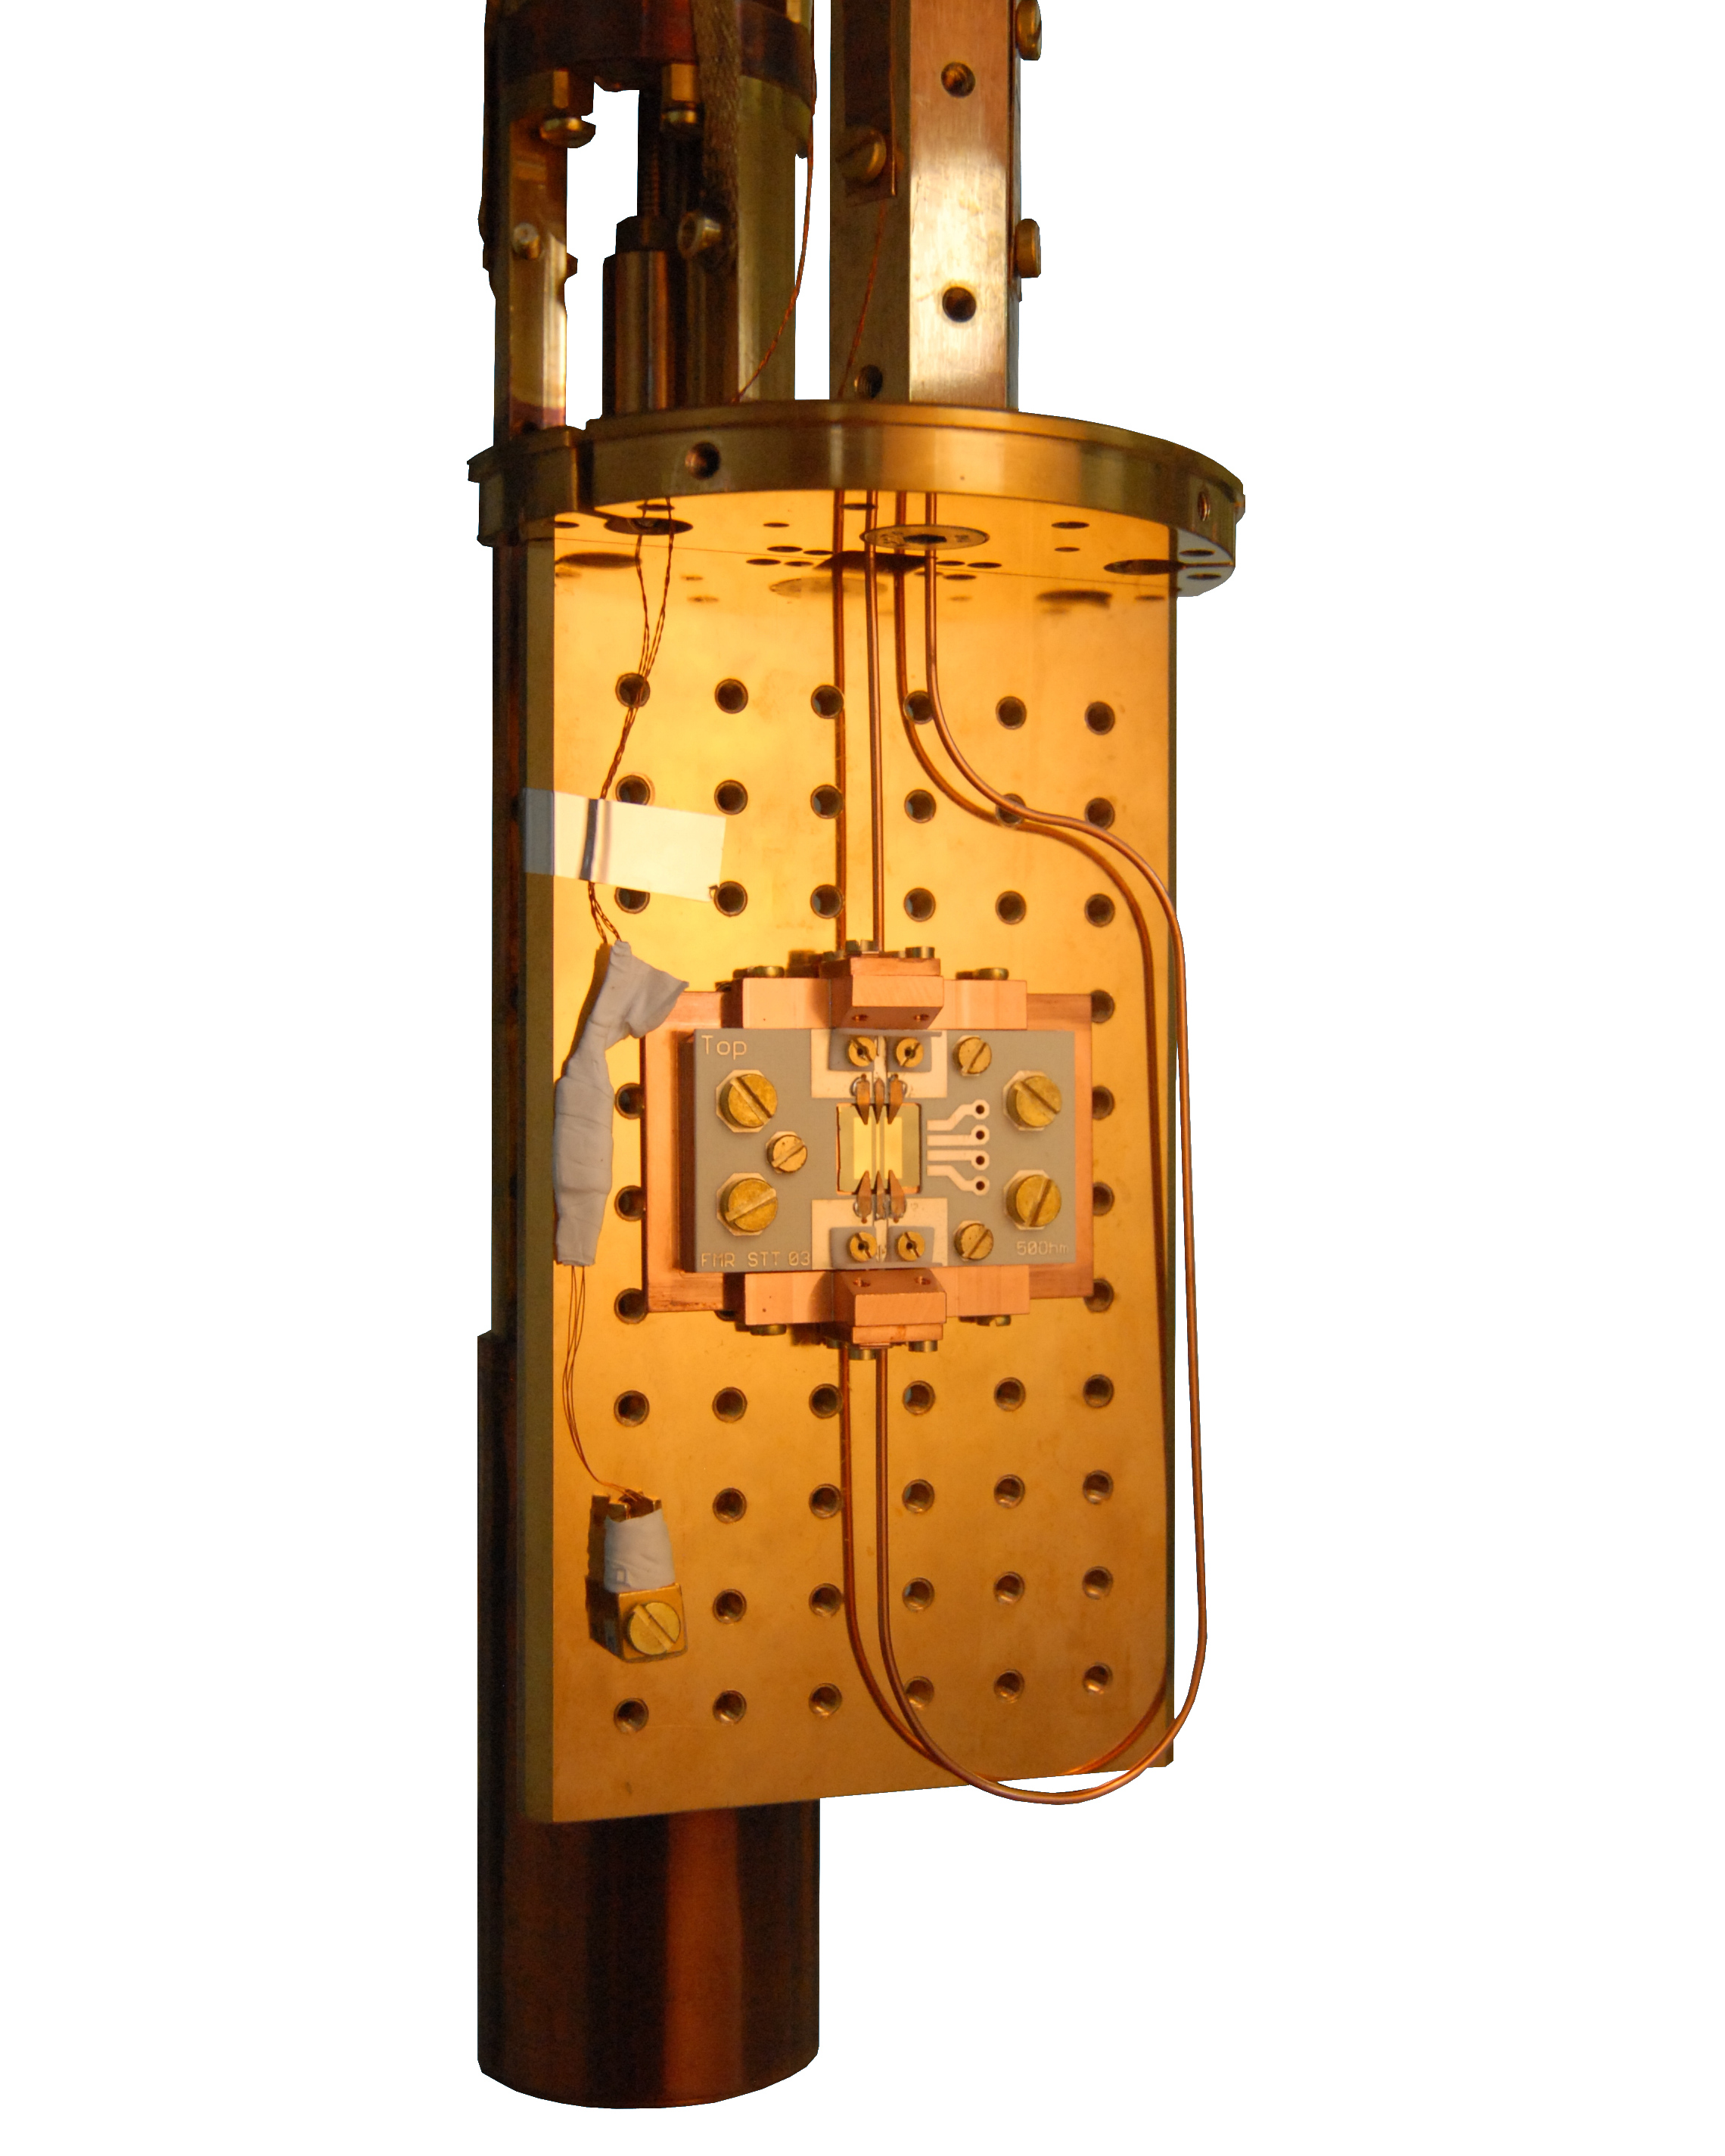
\includegraphics[width=\textwidth]{setup/holder/BF_freecut_45.jpg}
         \caption{BlueFors setup sample holder}
         \label{fig:setup_photo_bluefors}
     \end{subfigure}
     \begin{subfigure}[b]{.45\textwidth}
         \centering
         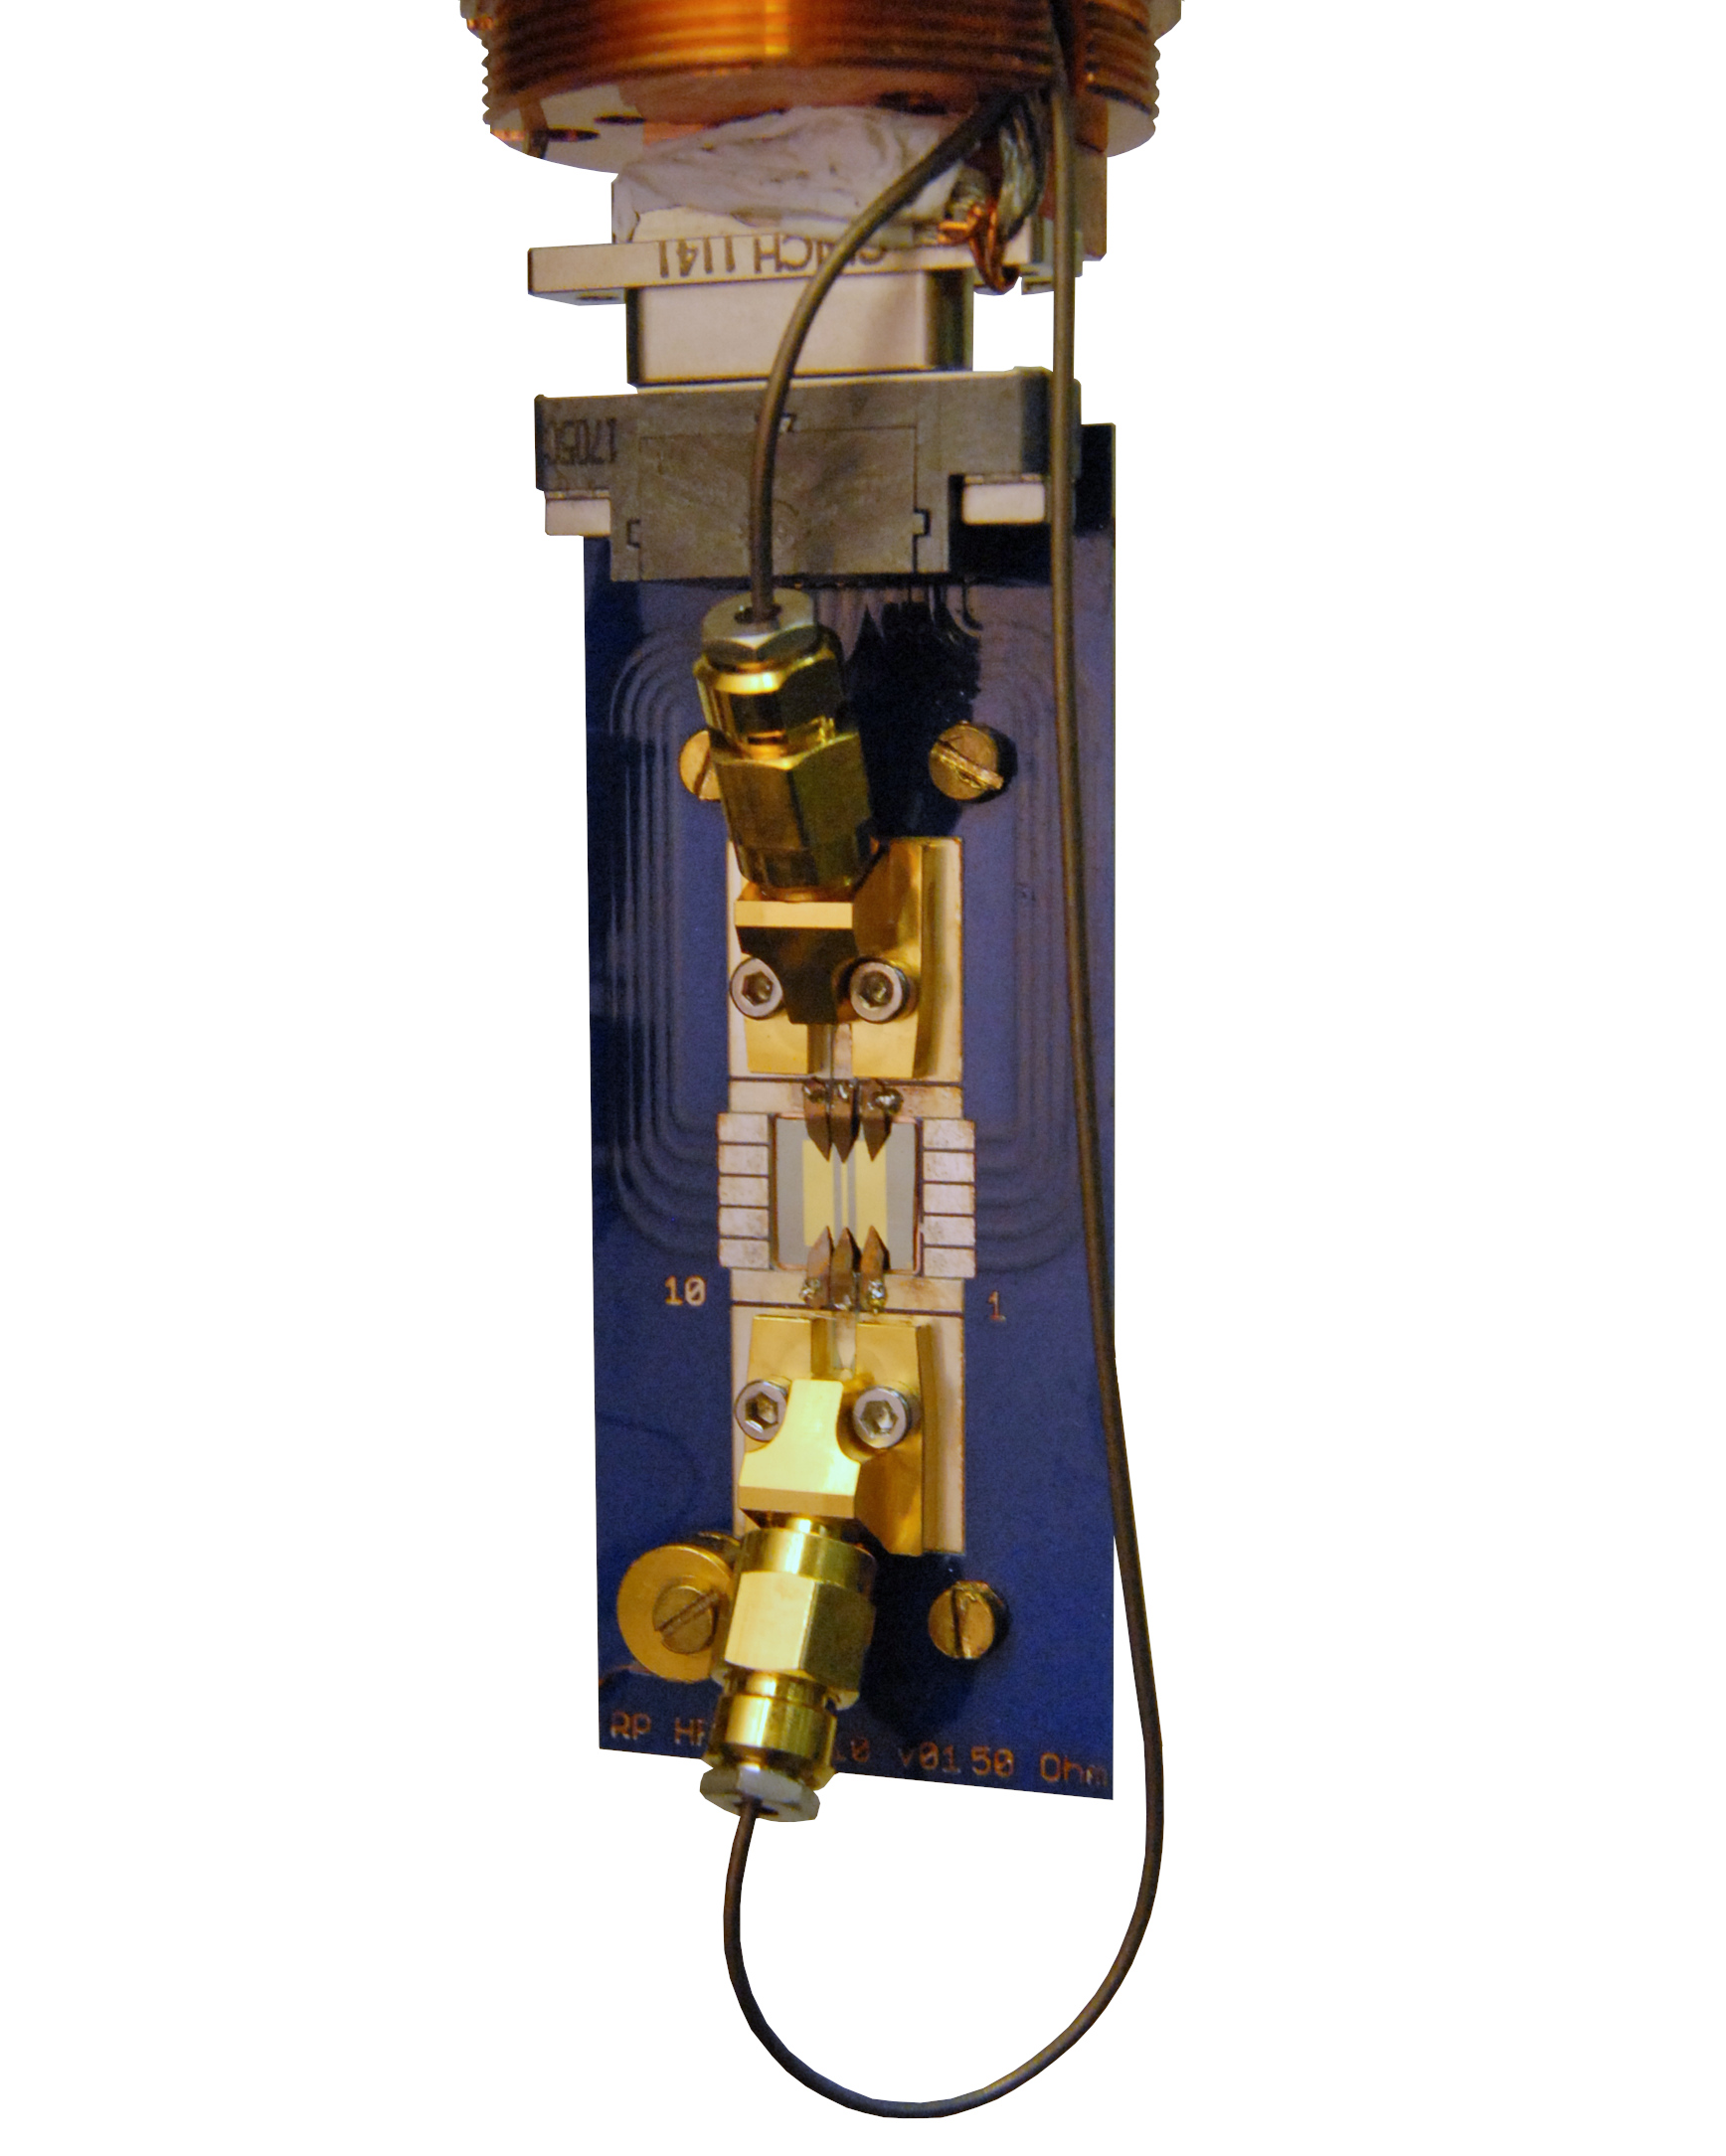
\includegraphics[width=\textwidth]{setup/holder/FH_freecut.jpg}
         \caption{HelioxVL setup sample holder}
         \label{fig:setup_photo_heliox}
     \end{subfigure}
        \caption[Sample holder pictures]{Sample holder pictures. \textbf{(a)} shows the FMR sample holder, with the mechanically controlled break junction setup in the background. Sample CPW3 is mounted. On the left side of the plate, the thermometer for $T_\text{FMR}$ is installed. \textbf{(b)} shows the sample holder of the Heliox setup. Beside the wave guide clamps, there are also bonding pads for direct current measurements. Again in the lower left, you can see the thermometer $T_\text{FMR}$ without any cables connected.}
        \label{fig:setup_photo}
\end{figure}

The HelioxVL setup in a wet cryostats, consisting of a $^3$He sample-in-vacuum dipstick and a dewar with built-in superconducting magnet. A thermometer is attached to the sample holder. The high-frequency cabling and the sample holder shown in Figure \ref{fig:setup_photo}b were realized in advance by Andreas Bloch and Lukas Kammermeier. The high-frequency cabling consist of copper cables for all setup parts with operating temperatures down to $4\,$K. For all parts with lower operating temperatures superconducting high frequency cables consisting of Nb/Ti are used.

The vector network analyzer (VNA) and pre-amplifier are mounted on a mobile rack for easy switching between setups. In addition, the room temperature thermometer and a measurement PC are mounted.

The VNA, both magnets, the room temperature thermometer and the thermometer of the HelioxVL Setup are controlled by the self-written program 'FMR control'. It is written in python3 and is mainly based on the packages pyvisa, numpy and matplotlib. It consists out of self-written device drivers and one central control program. By those drivers, the user can communicate with and control the devices. Several security features are implemented in them as well. Some device drivers can be found in the Appendix.

The measurement itself is run as multi-threading program, since recording the temperature, VNA and magnet control have to be done simultaneous. In general, at least one thread is recording the temperature the whole time. The logged temperature is averaged and then updated in a text file with corresponding timestamp. Another thread is controlling the magnet and VNA iteratively. Each iteration conducts the following operations. First, the magnet ramps to the desired field. Then the VNA measures the scattering parameter for all desired frequencies. A text file with the magnetic field, a timestamp and all the scattering parameter values and frequencies are saved. Afterwards these operations are conducted for the next desired magnetic field.